\documentclass[12pt]{article}
\usepackage{unicode-math}
\setmainfont
[    Extension = .otf,
   UprightFont = *-regular,
      BoldFont = *-bold,
    ItalicFont = *-italic,
BoldItalicFont = *-bolditalic,
]{xits}

\setmathfont
[    Extension = .otf,
      BoldFont = *bold,
]{xits-math}
\usepackage[scaled=.95]{sourcecodepro}
\usepackage{polyglossia}
\usepackage{verbatim}
\usepackage{graphicx}
\usepackage{hyperref}
\usepackage[margin=13mm]{geometry}
\setmainlanguage{russian}
\begin{document}
\title{Отчет по дисциплине <<Статистические пакеты>>}
\author{Выполнил: студент группы 09--616 Галанин Дмитрий \and Преподаватель: Заикин Артем Александрович}
\date{18. 12. 2016}
\maketitle
\section{Постановка задачи}
Исходные данные представляют собой набор из 15120 наблюдений следующего вида: каждое наблюдение - участок леса размером $30 \times 30$ метров из Национального Леса имени Рузвельта.

Описание полей:
\begin{itemize}
	\item Elevation --- средняя высота над уровнем моря,
	\item Aspect --- азимут направления самого крутого спуска на участке,
	\item Slope --- подъем в градусах,
	\item Horizontal\_Distance\_To\_Hydrology --- горизонтальное расстояние до ближайшего источника воды,
	\item Vertical\_Distance\_To\_Hydrology --- вертикальное расстояние до ближайшего источника воды,
	\item Horizontal\_Distance\_To\_Roadways --- горизонтальное расстояние до ближайшей дороги,
	\item Hillshade\_9am (0 to 255 index) --- количество тени в 9:00,
	\item Hillshade\_Noon (0 to 255 index) --- количество тени в 12:00,
	\item Hillshade\_3pm (0 to 255 index) --- количество тени в 15:00,
	\item Horizontal\_Distance\_To\_Fire\_Points --- горизонтальное расстояние до ближайшего участка распространения огня,
	\item Wilderness\_Area (4 бинарных показателя) --- категория дикости местности,
	\item Soil\_Type (40 бинарных показателей) --- тип почвы,
	\item Cover\_Type* (7 типов, указаны целым числом от 1 до 7) --- тип лесного покрова.
\end{itemize}
Задачей является построение регрессии переменной Cover\_Type.
\section{Анализ и обработка данных}
Вначале, после загрузки набора данных (<<датафрейма>>, англ. \textit{dataframe})
выполним преобразование бинарных показателей (а также переменной Cover\_Type) в категориальные переменные.
(Создаются новые столбцы Soil\_Type и Wilderness\_Area, содержащие в числовом виде тип (категорию) переменной вместо
бинарных показателей, после чего <<старые>> столбцы удаляются. Это упростит нам запись формул при создании моделей.)

Анализ данных с помощью функций типа \verb|boxplot()| показывает, что <<выбросов>> (англ. \textit{outliers}) нет или
имеется достаточно небольшое количество (не более 5,5\%; результаты представлены в таблице),
что не должно сказаться на точности получаемых моделей.

\begin{tabular}{|l|r|}
	\hline
	Переменная                   & Число <<выбросов>> \\ \hline
	Elevation                              & 0                               \\
	Aspect                                 & 0                               \\
	Slope                                  & 57                              \\
	Horizontal\_Distance\_To\_Hydrology    & 512                             \\
	Vertical\_Distance\_To\_Hydrology      & 586                             \\
	Horizontal\_Distance\_To\_Roadways     & 830                             \\
	Hillshade\_9am                         & 408                             \\
	Hillshade\_Noon                        & 393                             \\
	Hillshade\_3pm                         & 124                             \\
	Horizontal\_Distance\_To\_Fire\_Points & 645                             \\ \hline
\end{tabular}

\section{Выбор моделей}
В нашем примере зависимая переменная является категориальной. Поэтому при построении моделей будем использовать логистическую
регрессию (параметр \verb|family=poisson(link="log")|).

Вначале необходимо <<отсеять>> переменные, от которых (с большой вероятностью) не зависит наша переменная Cover\_Type. Для этого
используем GLM с формулой вида \verb|Cover_Type ~ .|:

(Точка в формуле после тильды обозначает зависимость от всех остальных (не указанных явно) переменных).

Далее по значениям тестовой $z$-статистики (и вероятности подтверждения гипотезы $H_0$, утверждающей о том, что коэффициент при
данной переменной-регрессоре в модели равен 0, т. е. зависимость фактически отсутствует) выбираем существенные переменные в модели.


Следует заметить, что графики, как правило, предназначены для линейных регрессионных моделей и не имеют смысла для логистических
(см. также здесь:\\ http://stats.stackexchange.com/questions/121490/interpretation-of-plotglm-model).
Поэтому для валидации модели обратимся непосредственно к численным данным (функции \verb|summary()|)
\begin{verbatim}
Call:
glm(formula = Cover_Type ~ Elevation + Aspect + Hillshade_9am +
    Hillshade_Noon + Soil_Type + Horizontal_Distance_To_Fire_Points +
    Wilderness_Area, family = poisson(link = "log"), data = df)

Deviance Residuals:
    Min       1Q   Median       3Q      Max
-2.9961  -0.6153  -0.0370   0.4909   3.1695

Coefficients:
                                     Estimate Std. Error z value Pr(>|z|)
(Intercept)                         1.835e+00  9.677e-02  18.962  < 2e-16 ***
Elevation                          -3.259e-04  3.231e-05 -10.084  < 2e-16 ***
Aspect                              1.780e-04  5.091e-05   3.496 0.000473 ***
Hillshade_9am                       1.301e-03  1.937e-04   6.716 1.87e-11 ***
Hillshade_Noon                     -7.732e-04  2.193e-04  -3.526 0.000423 ***
Soil_Type2                          2.240e-02  3.368e-02   0.665 0.505951
Soil_Type3                         -9.175e-02  3.101e-02  -2.958 0.003093 **
Soil_Type4                         -9.774e-02  3.363e-02  -2.906 0.003656 **
Soil_Type5                          9.782e-02  4.514e-02   2.167 0.030253 *
Soil_Type6                          4.303e-02  3.314e-02   1.298 0.194169
Soil_Type8                         -4.170e-01  7.082e-01  -0.589 0.555988
Soil_Type9                         -5.008e-01  2.322e-01  -2.157 0.031013 *
Soil_Type10                         1.508e-01  2.943e-02   5.123 3.00e-07 ***
Soil_Type11                         2.243e-02  3.828e-02   0.586 0.557867
Soil_Type12                        -4.762e-01  6.047e-02  -7.875 3.42e-15 ***
Soil_Type13                         1.278e-01  3.867e-02   3.304 0.000954 ***
Soil_Type14                         6.239e-02  4.493e-02   1.388 0.165011
Soil_Type16                         7.981e-02  5.338e-02   1.495 0.134832
Soil_Type17                         6.346e-02  3.293e-02   1.927 0.053982 .
Soil_Type18                         1.957e-01  7.365e-02   2.657 0.007892 **
Soil_Type19                        -1.356e-01  9.385e-02  -1.445 0.148359
Soil_Type20                        -1.864e-01  5.933e-02  -3.141 0.001685 **
Soil_Type21                        -3.239e-01  1.624e-01  -1.995 0.046080 *
Soil_Type22                        -7.245e-01  5.878e-02 -12.326  < 2e-16 ***
Soil_Type23                        -1.994e-01  4.179e-02  -4.771 1.83e-06 ***
Soil_Type24                        -3.293e-01  5.330e-02  -6.179 6.45e-10 ***
Soil_Type25                        -4.837e-01  7.086e-01  -0.683 0.494826
Soil_Type26                        -1.308e-01  8.028e-02  -1.630 0.103195
Soil_Type27                        -2.788e-01  1.668e-01  -1.671 0.094640 .
Soil_Type28                        -2.110e-01  1.956e-01  -1.079 0.280648
Soil_Type29                        -1.074e-01  4.195e-02  -2.560 0.010464 *
Soil_Type30                         2.796e-01  4.150e-02   6.736 1.63e-11 ***
Soil_Type31                        -2.225e-01  4.674e-02  -4.760 1.93e-06 ***
Soil_Type32                        -2.542e-01  4.160e-02  -6.111 9.91e-10 ***
Soil_Type33                        -1.327e-01  4.071e-02  -3.259 0.001119 **
Soil_Type34                         3.175e-02  1.142e-01   0.278 0.780940
Soil_Type35                         7.891e-01  5.562e-02  14.187  < 2e-16 ***
Soil_Type36                         6.155e-01  1.356e-01   4.539 5.66e-06 ***
Soil_Type37                         9.807e-01  7.883e-02  12.440  < 2e-16 ***
Soil_Type38                         7.302e-01  4.319e-02  16.906  < 2e-16 ***
Soil_Type39                         6.998e-01  4.348e-02  16.097  < 2e-16 ***
Soil_Type40                         7.741e-01  4.733e-02  16.355  < 2e-16 ***
Horizontal_Distance_To_Fire_Points  1.808e-05  4.949e-06   3.653 0.000259 ***
Wilderness_Area2                    1.570e-01  2.830e-02   5.547 2.91e-08 ***
Wilderness_Area3                    2.923e-01  1.880e-02  15.544  < 2e-16 ***
Wilderness_Area4                    1.444e-01  2.603e-02   5.549 2.88e-08 ***
---
Signif. codes:  0 ‘***’ 0.001 ‘**’ 0.01 ‘*’ 0.05 ‘.’ 0.1 ‘ ’ 1

(Dispersion parameter for poisson family taken to be 1)

    Null deviance: 16546  on 15119  degrees of freedom
Residual deviance: 10543  on 15074  degrees of freedom
AIC: 57760

Number of Fisher Scoring iterations: 5
\end{verbatim}
Зедсь уже видно, что данная модель не имеет проблем --- все переменные значимы (p-values для них достаточно малы;
переменная Soil\_Type же являеся категориальной), значение
Residual Deviance адекватно (значение \verb|pchisq(10543, 15074)| пренебрежимо мало --- $7.1 \times 10^{-189}$).
Кроме того, с потерей всего 45 ($15119-15074$) степеней свободы отклонение существенно (на 36.3\%, с 16546 до 10543) уменьшилось.
Поэтому мы можем точно сказать. что принимаем данную модель.

Рассмотрим также модель GAM (для нее пришлось исключить еще часть предположительно незначимых переменных, а также ввести гладкость
по переменной Elevation):
\begin{verbatim}
Family: poisson
Link function: log

Formula:
Cover_Type ~ s(Elevation) + Aspect + Vertical_Distance_To_Hydrology +
    Hillshade_Noon + Hillshade_3pm + Wilderness_Area

Parametric coefficients:
                                 Estimate Std. Error z value Pr(>|z|)
(Intercept)                     1.686e+00  4.465e-02  37.759  < 2e-16 ***
Aspect                          1.295e-04  4.839e-05   2.676  0.00745 **
Vertical_Distance_To_Hydrology -4.712e-04  7.228e-05  -6.519 7.09e-11 ***
Hillshade_Noon                 -1.901e-03  2.318e-04  -8.201 2.39e-16 ***
Hillshade_3pm                  -3.033e-04  1.379e-04  -2.200  0.02782 *
Wilderness_Area2               -7.981e-02  2.571e-02  -3.105  0.00190 **
Wilderness_Area3                1.577e-01  1.194e-02  13.207  < 2e-16 ***
Wilderness_Area4                1.251e-01  2.706e-02   4.623 3.78e-06 ***
---
Signif. codes:  0 ‘***’ 0.001 ‘**’ 0.01 ‘*’ 0.05 ‘.’ 0.1 ‘ ’ 1

Approximate significance of smooth terms:
               edf Ref.df Chi.sq p-value
s(Elevation) 8.981      9   4957  <2e-16 ***
---
Signif. codes:  0 ‘***’ 0.001 ‘**’ 0.01 ‘*’ 0.05 ‘.’ 0.1 ‘ ’ 1

R-sq.(adj) =  0.391   Deviance explained = 38.9%
UBRE = -0.32875  Scale est. = 1         n = 15120
\end{verbatim}
\begin{figure}
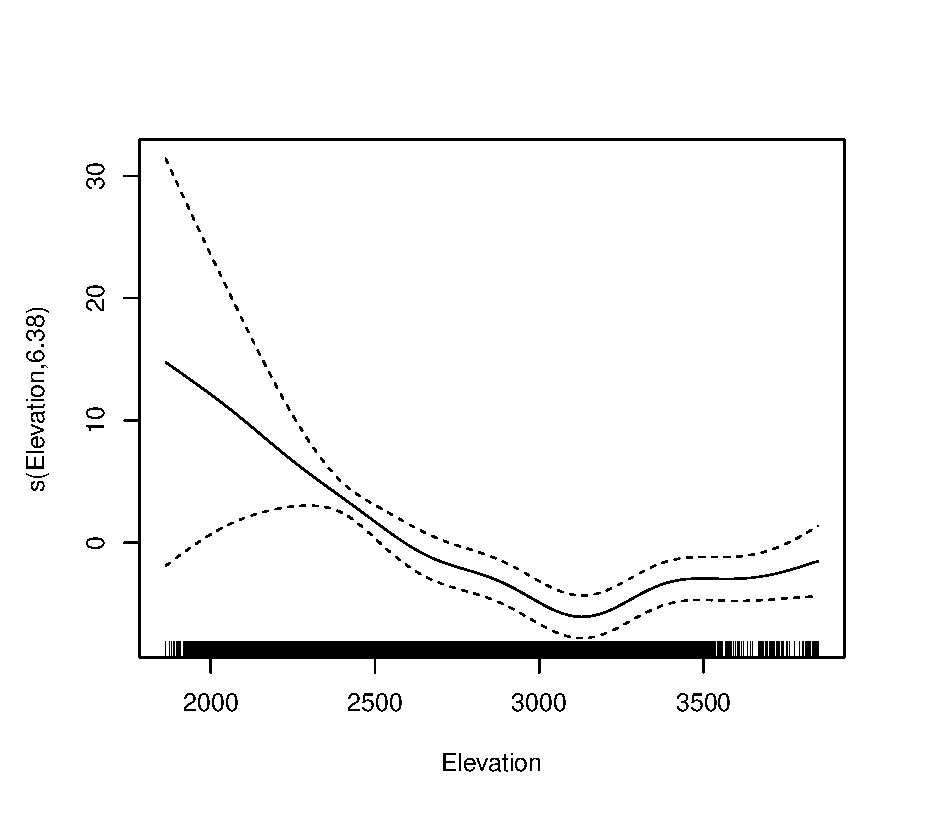
\includegraphics{gam1}
\caption{Пуассоновская GAM-модель}
\end{figure}
AIC данной модели равен 57273.77.

Как видим, GAM-модель также годится для описания зависимой переменной Cover\_Type.

Рассмотрим также GAM-модель с мультиномиальной моделью регрессии:
(\verb|family=multinom(K=6)|; всего имеется $7 = 6 + 1$ категория)

\begin{verbatim}
Family: multinom
Link function:

Formula:
Cover_Type ~ s(Elevation) + Aspect + Vertical_Distance_To_Hydrology +
    Hillshade_Noon + Hillshade_3pm + Wilderness_Area
~s(Elevation) + Aspect + Vertical_Distance_To_Hydrology + Hillshade_Noon +
    Hillshade_3pm + Wilderness_Area
~s(Elevation) + Aspect + Vertical_Distance_To_Hydrology + Hillshade_Noon +
    Hillshade_3pm + Wilderness_Area
~s(Elevation) + Aspect + Vertical_Distance_To_Hydrology + Hillshade_Noon +
    Hillshade_3pm + Wilderness_Area
~s(Elevation) + Aspect + Vertical_Distance_To_Hydrology + Hillshade_Noon +
    Hillshade_3pm + Wilderness_Area
~s(Elevation) + Aspect + Vertical_Distance_To_Hydrology + Hillshade_Noon +
    Hillshade_3pm + Wilderness_Area

Parametric coefficients:
                                   Estimate Std. Error z value Pr(>|z|)
(Intercept)                      -3.174e+00  1.078e+00  -2.945 0.003232 **
Aspect                            1.860e-04  4.371e-04   0.426 0.670390
Vertical_Distance_To_Hydrology    7.983e-03  7.075e-04  11.283  < 2e-16 ***
Hillshade_Noon                    2.872e-02  2.662e-03  10.789  < 2e-16 ***
Hillshade_3pm                    -7.054e-03  1.617e-03  -4.362 1.29e-05 ***
Wilderness_Area2                  6.055e-01  1.723e-01   3.513 0.000443 ***
Wilderness_Area3                 -3.152e-02  7.856e-02  -0.401 0.688225
Wilderness_Area4                  1.604e+01  3.682e+03   0.004 0.996524
(Intercept).1                    -3.467e+01  3.441e+03  -0.010 0.991960
Aspect.1                          6.790e-03  8.353e-04   8.129 4.34e-16 ***
Vertical_Distance_To_Hydrology.1  2.835e-02  1.449e-03  19.563  < 2e-16 ***
Hillshade_Noon.1                  4.816e-02  4.461e-03  10.797  < 2e-16 ***
Hillshade_3pm.1                  -3.871e-02  2.775e-03 -13.946  < 2e-16 ***
Wilderness_Area2.1               -3.275e+01  6.987e+14   0.000 1.000000
Wilderness_Area3.1                2.384e+01  3.441e+03   0.007 0.994472
Wilderness_Area4.1                3.800e+01  5.039e+03   0.008 0.993983
(Intercept).2                    -4.834e+01  1.603e+04  -0.003 0.997593
Aspect.2                          5.917e-03  9.426e-04   6.277 3.46e-10 ***
Vertical_Distance_To_Hydrology.2  1.910e-02  1.616e-03  11.822  < 2e-16 ***
Hillshade_Noon.2                  1.085e-01  5.097e-03  21.287  < 2e-16 ***
Hillshade_3pm.2                  -6.817e-02  3.036e-03 -22.452  < 2e-16 ***
Wilderness_Area2.2               -1.983e+01  9.809e+13   0.000 1.000000
Wilderness_Area3.2               -7.227e+01  5.001e+19   0.000 1.000000
Wilderness_Area4.2                3.808e+01  1.644e+04   0.002 0.998153
(Intercept).3                    -1.127e+01  1.901e+00  -5.930 3.03e-09 ***
Aspect.3                          4.699e-03  5.939e-04   7.912 2.53e-15 ***
Vertical_Distance_To_Hydrology.3  1.012e-02  9.235e-04  10.956  < 2e-16 ***
Hillshade_Noon.3                  4.711e-02  3.330e-03  14.147  < 2e-16 ***
Hillshade_3pm.3                  -3.299e-02  2.077e-03 -15.883  < 2e-16 ***
Wilderness_Area2.3               -6.673e+01  1.222e+15   0.000 1.000000
Wilderness_Area3.3                1.043e+00  1.054e-01   9.895  < 2e-16 ***
Wilderness_Area4.3               -4.636e+01  8.356e+12   0.000 1.000000
(Intercept).4                    -2.670e+01  3.096e+03  -0.009 0.993119
Aspect.4                          6.357e-03  8.150e-04   7.800 6.18e-15 ***
Vertical_Distance_To_Hydrology.4  1.918e-02  1.441e-03  13.307  < 2e-16 ***
Hillshade_Noon.4                  1.358e-02  4.381e-03   3.100 0.001934 **
Hillshade_3pm.4                  -2.437e-02  2.740e-03  -8.893  < 2e-16 ***
Wilderness_Area2.4               -5.108e-01  1.550e+07   0.000 1.000000
Wilderness_Area3.4                2.379e+01  3.096e+03   0.008 0.993870
Wilderness_Area4.4                3.792e+01  4.811e+03   0.008 0.993711
(Intercept).5                    -2.928e+00  2.233e+00  -1.311 0.189833
Aspect.5                          5.673e-04  5.330e-04   1.064 0.287218
Vertical_Distance_To_Hydrology.5 -5.349e-03  7.677e-04  -6.968 3.22e-12 ***
Hillshade_Noon.5                  7.485e-04  3.105e-03   0.241 0.809512
Hillshade_3pm.5                  -1.679e-02  2.001e-03  -8.389  < 2e-16 ***
Wilderness_Area2.5               -9.911e-01  1.651e-01  -6.002 1.95e-09 ***
Wilderness_Area3.5                6.996e-01  1.030e-01   6.792 1.11e-11 ***
Wilderness_Area4.5               -3.830e+01  3.378e+13   0.000 1.000000
---
Signif. codes:  0 ‘***’ 0.001 ‘**’ 0.01 ‘*’ 0.05 ‘.’ 0.1 ‘ ’ 1

Approximate significance of smooth terms:
                 edf Ref.df  Chi.sq  p-value
s(Elevation)   7.602  8.102  971.32  < 2e-16 ***
s.1(Elevation) 4.684  5.112  185.32  < 2e-16 ***
s.2(Elevation) 1.824  1.974   18.52 6.93e-05 ***
s.3(Elevation) 4.114  4.549  761.87  < 2e-16 ***
s.4(Elevation) 5.453  5.734  288.90  < 2e-16 ***
s.5(Elevation) 3.859  4.502 1052.70  < 2e-16 ***
---
Signif. codes:  0 ‘***’ 0.001 ‘**’ 0.01 ‘*’ 0.05 ‘.’ 0.1 ‘ ’ 1

Deviance explained = 60.2%
-REML = 9650.9  Scale est. = 1         n = 15120
\end{verbatim}

AIC данной модели равен 19240.19, что в 4 раза меньше предыдущих --- делаем
вывод, что данная модель подходит нам больше всего.
\begin{figure}
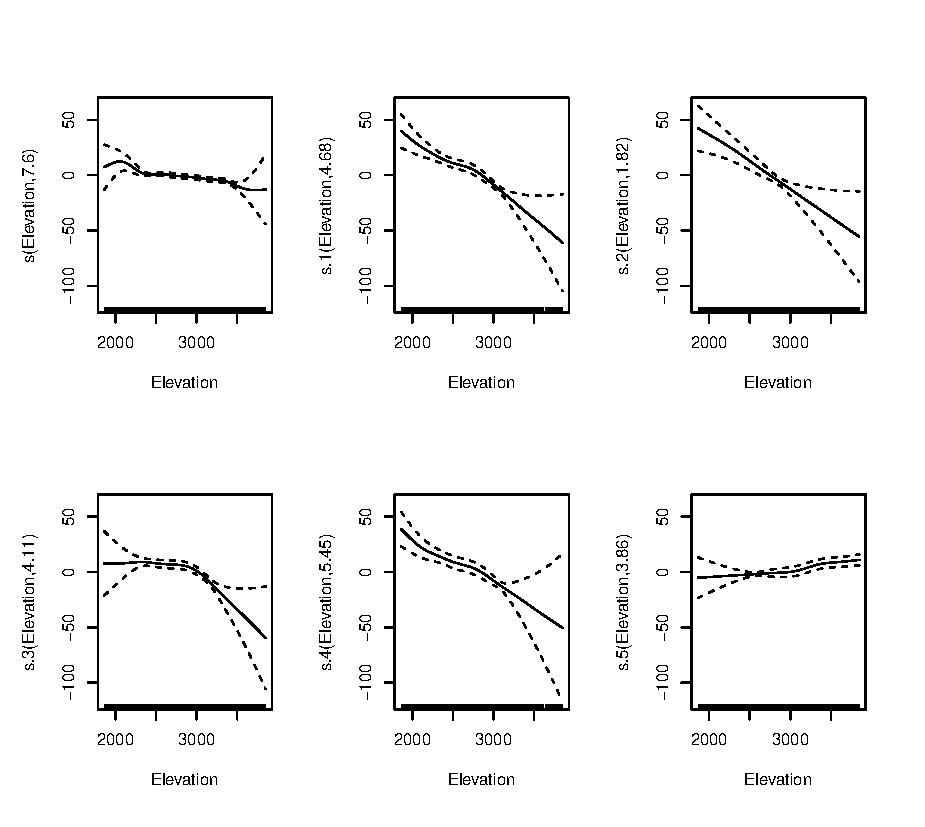
\includegraphics{gam2}
\caption{Мультиномиальная GAM-модель}
\end{figure}
\newpage
\section{Листинг кода на R}
\verbatiminput{../forests.r}
\end{document}
